\documentclass[
    12pt, 
    openright, 
    oneside, 
    a4paper, 
    chapter=TITLE, % --- Força título em caixa alta
    sumario=tradicional, % --- espaçamento padrão UEMA
    english, 
    brazil 
]{abntex2}

\usepackage{uema-style}

% --- Importa metadados do documento ---
\titulo{TÍTULO DA PROPOSTA TECNOLÓGICA}
\autor{NOME DO ALUNO 1\\NOME DO ALUNO 2\\NOME DO ALUNO 3}
\local{Apicum-Açu/MA}
\data{2026}
\orientador{Prof. Marcio Franklin Monteiro Souza}
\instituicao{
  UNIVERSIDADE ESTADUAL DO MARANHÃO
  \par
  NÚCLEO DE TECNOLOGIAS PARA EDUCAÇÃO
  \par
  CURSO TECNOLOGIA EM ANÁLISE E DESENVOLVIMENTO DE SISTEMAS
}
\tipotrabalho{Proposta Tecnológica}
\preambulo{Proposta Tecnológica apresentada ao Curso Superior de Tecnologia em Análise e Desenvolvimento de Sistemas, Universidade Estadual do Maranhão, Núcleo de Tecnologias para Educação, como componente curricular para obtenção do grau de Tecnólogo.}


% --- Configurações UEMA ---
% --- Configurações de Fonte ---
\usepackage{mathptmx} % Aplica a fonte Times New Roman

% --- Padronização de Títulos para Tamanho 12 e Fonte Times ---
\renewcommand{\ABNTEXchapterfont}{\bfseries}
\renewcommand{\ABNTEXchapterfontsize}{\normalsize}
\renewcommand{\ABNTEXsectionfont}{\bfseries}
\renewcommand{\ABNTEXsectionfontsize}{\normalsize}
\renewcommand{\ABNTEXsubsectionfont}{\bfseries}
\renewcommand{\ABNTEXsubsectionfontsize}{\normalsize}
\renewcommand{\ABNTEXsubsubsectionfont}{\bfseries}
\renewcommand{\ABNTEXsubsubsectionfontsize}{\normalsize}

% --- Ajuste de Espaçamento entre Títulos e Texto ---
\setlength{\afterchapskip}{1cm}  % Reduz o espaço logo abaixo dos títulos de capítulo
\setlength{\beforechapskip}{0cm}   % Ajusta o topo do capítulo

\setsecnumdepth{subsection}
\setcounter{secnumdepth}{3}

% Configuração das margens (UEMA: Superior 3cm, Esquerda 3cm, Inferior 2cm, Direita 2cm)
\setlrmarginsandblock{3cm}{2cm}{*}
\setulmarginsandblock{3cm}{2cm}{*}
\checkandfixthelayout

% --- Configuração de Listas (Padrão UEMA: Marcadores a, b, c e recuo de 2cm) ---
\usepackage{enumitem}

\setlist[enumerate,1]{
    label=\alph*),          % Define o marcador como a), b), c)...
    leftmargin=2.0cm,       % Aplica o recuo exato de 2cm na margem esquerda
    labelwidth=0.6cm,       % Largura reservada para a letra e o parêntese
    itemsep=0pt,            % Espaçamento entre os itens
    topsep=0pt              % Espaçamento acima da lista
}

\setlist[itemize]{
    leftmargin=2.0cm,       % Recuo de 2cm também para marcadores de lista com pontos
    itemsep=0pt,
    topsep=0pt
}


% --- Configuração Definitiva de Alíneas (Padrão UEMA) ---
\usepackage{enumitem}

\newlist{uemaenum}{enumerate}{1}
\setlist[uemaenum,1]{
    label=\alph*),
    leftmargin=2.75cm,
    labelsep=0.4cm,
    itemsep=2pt,
    topsep=2pt
}

% Para listas com marcadores (pontos), se precisar:
\newlist{uemaball}{itemize}{1}
\setlist[uemaball,1]{
    leftmargin=2.75cm,
    itemsep=2pt,
    topsep=2pt
}

% --- Redefinição da Capa para Tamanho 12 e alinhamentos UEMA ---
% --- Redefinição da Capa para Tamanho 12 e Título Centralizado Absoluto ---
\renewcommand{\imprimircapa}{%
  \begin{capa}%
    \center
    
    % 1. Bloco superior com altura fixa (ex: 7cm) para englobar os autores
    \begin{minipage}[t][7cm][t]{\textwidth}
        \centering
        \normalfont\normalsize
        \imprimirinstituicao
        
        \vspace*{3\baselineskip}
        \bfseries\normalsize
        \imprimirautor
    \end{minipage}
    
    % Mola de espaço flexível
    \vspace*{\fill}
    
    % 2. Título (ficará travado no centro exato da folha)
    \bfseries\normalsize\imprimirtitulo
    
    % Mola de espaço flexível
    \vspace*{\fill}
    
    % 3. Bloco inferior com exatamente a mesma altura do bloco superior (7cm)
    \begin{minipage}[b][7cm][b]{\textwidth}
        \centering
        \normalfont\normalsize
        \imprimirlocal\par
        \imprimirdata
    \end{minipage}
  \end{capa}
}
% --- Redefinição da Folha de Rosto para Tamanho 12 e Espaçamentos Exatos ---
\makeatletter
\renewcommand{\folhaderostocontent}{
  \begin{center}
    % 1. Autores (Na margem superior)
    \bfseries\normalsize\imprimirautor
    
    % 2. Título (Intervalo de 4 quebras de linha / cai na 5ª linha)
    \vspace*{4\baselineskip}
    \bfseries\normalsize\imprimirtitulo
  \end{center}
  
  % 3. Preâmbulo / Resuminho (Intervalo de 2 quebras de linha)
  \vspace*{2\baselineskip}
  
  % Anula o parágrafo e alinha a caixa perfeitamente à direita
  \noindent\hfill
  \begin{minipage}{0.5\textwidth}
      \normalfont\normalsize\SingleSpacing % Espaço simples
      \imprimirpreambulo
      \par\vspace*{\baselineskip} % 1 linha de espaço antes do orientador
      
      % Orientador sem negrito
      \imprimirorientadorRotulo~\imprimirorientador
  \end{minipage}
  
  % 4. Local e Data 
  \vspace*{\fill}
  
  \begin{center}
    \normalfont\normalsize
    \imprimirlocal\par
    \imprimirdata
  \end{center}
}
\makeatother
% --- Ajustes Finos do Sumário (Normas UEMA) ---

% 1. Remove TODOS os espaçamentos verticais extras (espaço 1.5 uniforme)
\setlength{\cftbeforechapterskip}{0pt}
\renewcommand{\insertchapterspace}{}

% 2. Deixa os pontinhos da linha mais juntos
\renewcommand{\cftdotsep}{2}
\renewcommand{\cftchapterdotsep}{2}
\renewcommand{\cftsectiondotsep}{2}
\renewcommand{\cftsubsectiondotsep}{2}
\renewcommand{\cftsubsubsectiondotsep}{2}

% 3. Alinha TODAS as seções e subseções rigorosamente à esquerda (margem 0)
\setlength{\cftchapterindent}{0pt}
\setlength{\cftsectionindent}{0pt}
\setlength{\cftsubsectionindent}{0pt}
\setlength{\cftsubsubsectionindent}{0pt}

% 4. Distância entre o número e o texto
\setlength{\cftchapternumwidth}{1.3cm}
\setlength{\cftsectionnumwidth}{1.3cm}
\setlength{\cftsubsectionnumwidth}{1.3cm}
\setlength{\cftsubsubsectionnumwidth}{1.3cm}

% 5. Força todas as subseções a ficarem em negrito
\renewcommand{\cftsectionfont}{\bfseries}
\renewcommand{\cftsubsectionfont}{\bfseries}
\renewcommand{\cftsubsubsectionfont}{\bfseries}

% 5. Números das páginas nunca em negrito
\renewcommand{\cftchapterpagefont}{\normalfont}
\renewcommand{\cftsectionpagefont}{\normalfont}
\renewcommand{\cftsubsectionpagefont}{\normalfont}
\renewcommand{\cftsubsubsectionpagefont}{\normalfont}
% =========================================================
% --- Formatação de Apêndices e Anexos (Padrão UEMA) ---
% =========================================================

% 1. Altera as folhas de divisão para CAIXA ALTA
\renewcommand{\apendicesname}{\textbf{APÊNDICES}}

% 2. Remove o negrito dos títulos de cada Apêndice individual
\let\oldapendicesenv\apendicesenv
\renewcommand{\apendicesenv}{%
    \oldapendicesenv
    % \normalfont remove o negrito; \raggedright trava na margem esquerda
    \renewcommand{\ABNTEXchapterfont}{\normalfont}
}

% 3. Espaçamentos
\makeatletter
\renewcommand{\partapendices}{%
  \cleardoublepage
  \thispagestyle{empty}%
  \vspace*{0.4\textheight}% Puxa exatamente para o meio vertical da página
  \begin{center}%
    \bfseries\normalsize\apendicesname%
  \end{center}%
  \newpage%
}
\makeatother
% --- Formatação de Anexos (Padrão UEMA) ---

% 1. Altera as folhas de divisão para CAIXA ALTA
\renewcommand{\anexosname}{\textbf{ANEXOS}}

% 2. Remove o negrito dos títulos de cada Anexo individual
\let\oldanexosenv\anexosenv
\renewcommand{\anexosenv}{%
    \oldanexosenv
    % \normalfont remove o negrito; \raggedright trava na margem esquerda
    \renewcommand{\ABNTEXchapterfont}{\normalfont}
}

% 3. Espaçamentos
\makeatletter
\renewcommand{\partanexos}{%
  \cleardoublepage
  \thispagestyle{empty}%
  \vspace*{0.4\textheight}%
  \begin{center}%
    \bfseries\normalsize\anexosname%
  \end{center}%
  \newpage%
}
\makeatother

\begin{document}
\selectlanguage{brazil}
\frenchspacing

% ----------------------------------------------------------
% ELEMENTOS PRÉ-TEXTUAIS
% ----------------------------------------------------------
\imprimircapa
\imprimirfolhaderosto

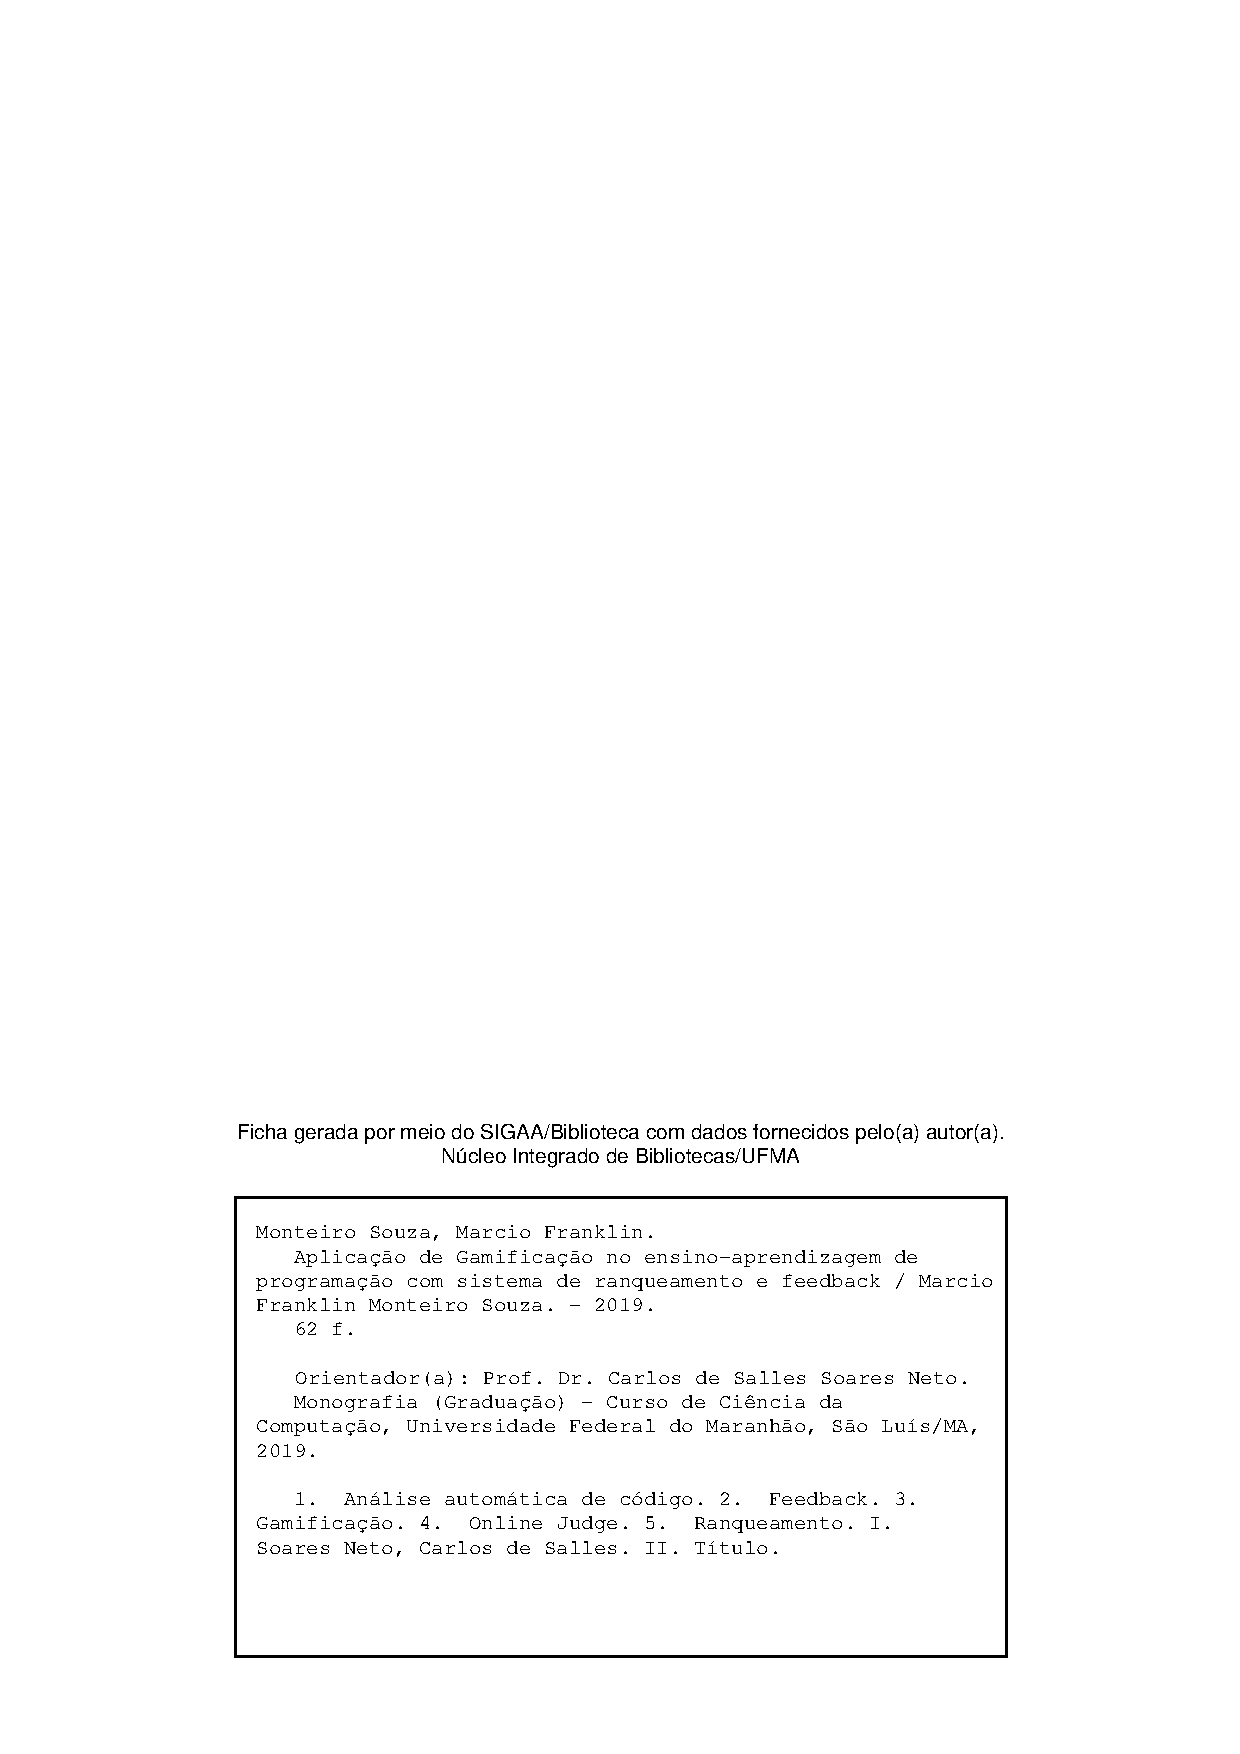
\includepdf[pages=-]{pdfs/ficha_catalografica.pdf}

\begin{folhadeaprovacao}
  % 1. Autor e Título na margem superior
  \begin{center}
    \bfseries\normalsize\imprimirautor\par
    \vspace*{2\baselineskip}
    \bfseries\normalsize\imprimirtitulo
  \end{center}
  
  \vspace*{\fill}
  
  % 2. Preâmbulo começando exatamente no eixo vertical da página
  \noindent\hfill
  \begin{minipage}{0.5\textwidth}
      \normalfont\normalsize\SingleSpacing
      \imprimirpreambulo
  \end{minipage}
  
  \vspace*{\fill}
  
  % 3. Data de aprovação alinhada à esquerda
  \noindent\normalfont\normalsize Aprovada em \_\_\_/\_\_\_/\_\_\_\_\_\_
  
  \vspace*{2\baselineskip}
  
  % 4. Título da Banca (centralizado)
  \begin{center}
    BANCA EXAMINADORA
  \end{center}
  
  % 5. Assinaturas
  \assinatura{
    \imprimirorientador\ (Orientador) \\ 
    Titulação em xxxxxxxxxxx \\ 
    Instituição da Titulação
  }
  
  \assinatura{
    Prof. Titulação Nome do examinador (Examinador 1) \\ 
    Titulação em xxxxxxxxxxx \\ 
    Instituição da Titulação
  }
  
  \assinatura{
    Prof. Titulação Nome do examinador (Examinador 2) \\ 
    Titulação em xxxxxxxxxxx \\ 
    Instituição da Titulação
  }
\end{folhadeaprovacao}
\setlength{\absparsep}{18pt}
\begin{resumo}
    A diretriz para a elaboração é a NBR 6028/21 segundo a ABNT. Resumo no formato informativo contendo: introdução e apresentação da temática. Apresentação dos objetivos geral e específicos. Metodologia. Resultados e discussão e conclusão. Deve ser no impessoal, na terceira pessoa do singular, na voz ativa com no mínimo 150 e máximo de 500 palavras. O resumo não apresenta nenhum tipo de recuo e nenhum parágrafo. Não deve conter citações. Utilizar tamanho da fonte 12 e espaçamento entre linhas 1,5. Logo após o resumo apresentar sequência de palavras que representam as categorias principais do trabalho que são conhecidas como palavras-chave, usar no mínimo três e no máximo cinco palavras, separadas entre si por ponto e vírgula e finalizadas por ponto. Devem ser grafadas com as iniciais em letra minúscula, exceto os substantivos próprios e nomes científicos, que aparecem com inicial maiúscula.
    
    Palavras-chave: resumo; ABNT; pesquisa.
\end{resumo}

\begin{resumo}[Abstract]
 \begin{otherlanguage*}{english}
    Reprodução do resumo em língua estrangeira, utilizando-se da mesma formatação.
    
    The guideline for elaboration is NBR 6028/93 according to ABNT. Summary in informative format containing: introduction and presentation of the theme. Presentation of general and specific objectives. Methodology. Results and discussion and conclusion. It must be impersonal, third person singular, active voice with a minimum of 150 and a maximum of 500 words.
    
    Keywords: summary; ABNT; search.
 \end{otherlanguage*}
\end{resumo}


% --- Sumário ---
\pdfbookmark[0]{\contentsname}{toc}
\tableofcontents*
\cleardoublepage

% ----------------------------------------------------------
% ELEMENTOS TEXTUAIS
% ----------------------------------------------------------
\textual

\chapter{JUSTIFICATIVA}
Na justificativa é necessário fazer uma breve apresentação da temática principal e colocar evidente o porquê da escolha do tema. Pode-se colocar impressões pessoais (sem usar a primeira pessoa do singular) que favorecerem desde a escolha do objeto de pesquisa até questões como se trabalhou, ou trabalha, no local a ser investigado.

Apresentar o problema a ser investigado (lembrando que tem que ser no formato de uma pergunta).

A pesquisa será norteada pelas hipóteses abaixo, sendo que no percurso de investigação elas serão refutadas ou confirmadas:
\begin{uemaenum}
    \item Descrição da Hipótese 1;
    \item Descrição da Hipótese 2;
    \item Descrição da Hipótese 3.
\end{uemaenum}

\chapter{OBJETIVOS}
São objetivos deste projeto:

\section{Geral}
Analisar...

\section{Específicos}
\begin{uemaenum}
    \item Identificar...;
    \item Diagnosticar...;
    \item Apresentar....
\end{uemaenum}

\chapter{REFERENCIAL TEÓRICO}
Nesta seção é apresentado um debate acerca do que os pesquisadores falam acerca do tema escolhido para a pesquisa. Privilegie o máximo de fontes diferentes (artigos, teses, dissertações, monografias e livros). Exemplo de citação \cite{towfic2022benchmarking}.

Segundo \citeonline{chu2021sustained}, isto é um outro exemplo de citação.

\begin{citacao}
Injeção de dependências (\textit{dependency injection} ou DI) é um padrão de
desenvolvimento de software usado para manter o baixo acoplamento entre classes do
sistema. As dependências de um objeto não são instanciadas programaticamente, mas
sim injetadas de alguma forma \cite{chambers2021macbook}.
\end{citacao}

\chapter{METODOLOGIA}
Nesta seção é apresentado o método e delimitada a metodologia (quanto à abordagem: quantitativa ou qualitativa; quanto aos objetivos: explicativa, descritiva ou exploratória; e, quanto aos procedimentos).

\begin{figure}[htb]
    \centering
	\caption{\label{fig:bpmn-modelagem}Representação da estrutura do Spring Data}
	% --- 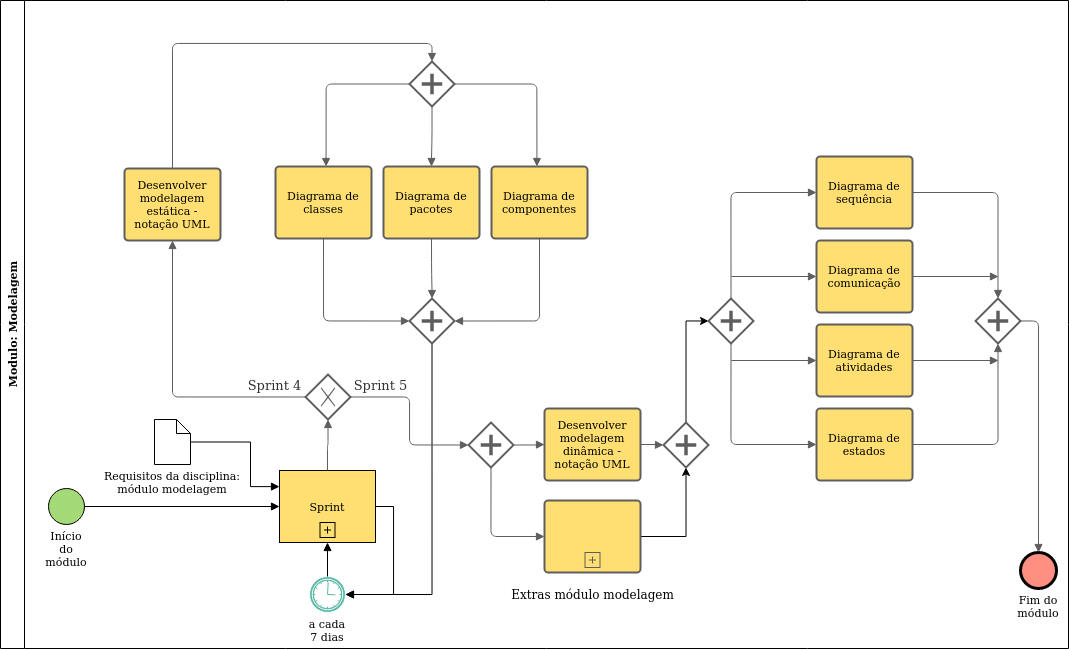
\includegraphics[scale=0.8]{img/bpmn_modelagem.png}
    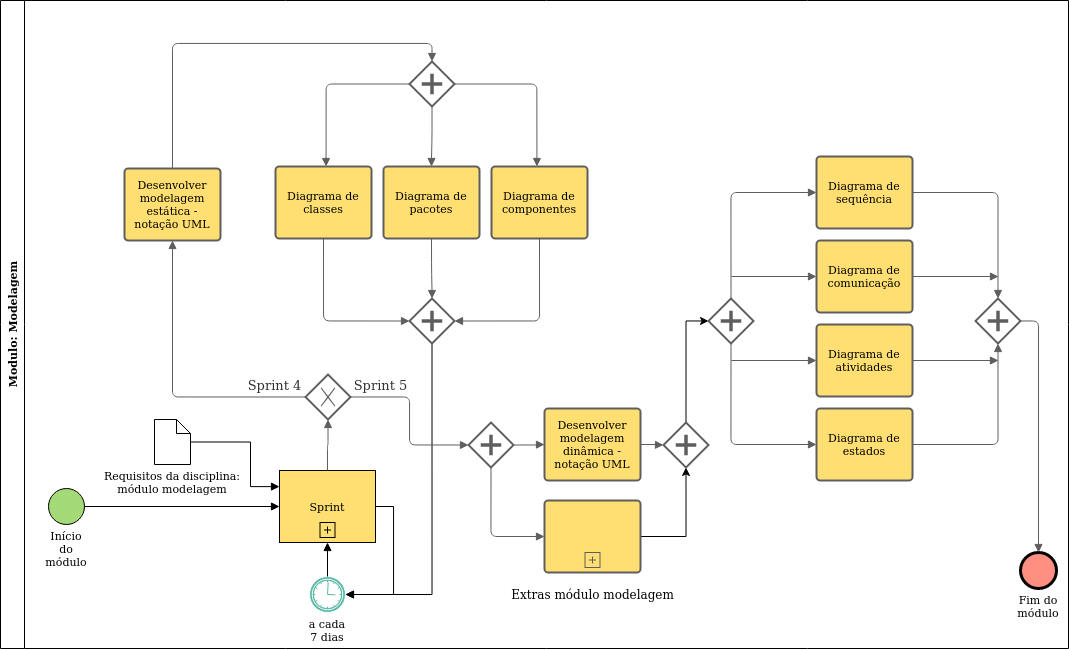
\includegraphics[width=0.85\linewidth]{img/bpmn_modelagem.png}
	\fonte{\citeonline{ribeiro2015beneficios}}
\end{figure}

\chapter{PROPOSTA TECNOLÓGICA}
Nesta seção serão apresentados os resultados obtidos e as soluções para o problema detectado de acordo com a natureza da proposta (diagnóstico, software, patente).
Nesta seção serão apresentados os resultados obtidos e as soluções para o problema detectado de acordo com a natureza da proposta (diagnóstico, software, patente).

Este é o exemplo de uso de notas de rodapé. O sistema foi desenvolvido utilizando a arquitetura de microsserviços\footnote{Para mais informações acesse: \url{https://aws.amazon.com/pt/microservices/}} para garantir maior escalabilidade.

\chapter{CRONOGRAMA}
\begin{table}[htb]
\centering
\caption{Cronograma de atividades}
\begin{tabular}{|l|c|c|c|c|c|c|c|}
\hline
\textbf{Atividades / Meses} & \textbf{Jun} & \textbf{Jul} & \textbf{Ago} & \textbf{Set} & \textbf{Out} & \textbf{Nov} & \textbf{Dez} \\ \hline
Levantamento bibliográfico & X & & & & & & \\ \hline
Elaboração do Projeto de Intervenção & X & X & & & & & \\ \hline
Pesquisa de campo & & & X & X & & & \\ \hline
Aplicação do instrumento & & & X & X & & & \\ \hline
Análise dos Dados & & & & X & X & & \\ \hline
Entrega do projeto & & & & & & X & \\ \hline
Elaboração da proposta & & & & & & X & \\ \hline
Apresentação & & & & & & & X \\ \hline
\end{tabular}
\fonte{Elaborado pelo autor (\the\year).}
\end{table}


% ----------------------------------------------------------
% ELEMENTOS PÓS-TEXTUAIS
% ----------------------------------------------------------
\postextual

\bibliography{bib/referencias}

\begin{apendicesenv}
\partapendices

\chapter{\raggedright TÍTULO DO APÊNDICE}
Insira aqui o seu apêndice (material complementar elaborado pelo próprio pesquisador).
\end{apendicesenv}

\begin{anexosenv}
\partanexos

\chapter{\raggedright TÍTULO DO ANEXO}

Insira aqui o seu anexo (material retirado de outras fontes).
\end{anexosenv}


\end{document}
